\documentclass{oci}
\usepackage[utf8]{inputenc}
\usepackage{lipsum}
\usepackage{amsmath}

\title{Burrito de letras}

\begin{document}
\begin{problemDescription}
  En el Instituto de Colección de Palabras en Cuadrículas (ICPC) son fanáticos
  de los juegos que involucran palabras tales como la famosa sopa de letras
  en donde un jugador debe buscar palabras ocultas en una cuadrícula de $n \times n$
  casillas.
  %
  Cada año, el ICPC organiza una convención donde se presentan
  innovadoras variantes de juegos de palabras.
  %
  Este año, Norma Gibat, la famosa inventora de juegos de palabra,
  presentó una nueva versión de la sopa de letras basándose en su
  comida favorita: los burritos.

  Esta nueva versión, llamada ``burrito de letras'', funciona igual
  que una sopa de letras normal, solo que además la cuadrícula es
  colocada alrededor de un cilindro como si estuviese envolviendo
  un burrito.
  %
  Específicamente, las reglas del burrito de letras son las siguientes:
  \begin{itemize}
    \item El juego consiste en una cuadrícula de $n \times n$ donde cada casilla tiene una letra
      escrita.
    \item Al jugador se le presenta además una lista de $m$ palabras, las cuales
      pueden estar o no escritas en la cuadrícula.
      %
      Para cada una de ellas, el jugador debe responder
      si está o no en la cuadrícula.
    \item Una palabra puede estar escrita en cualquier lugar de forma vertical de arriba hacia abajo,
      o de forma horizontal de izquierda a derecha.
      %
      Las palabras no pueden aparecer de forma diagonal.
    \item La cuadrícula está colocada alrededor de un cilindro y una palabra puede
      ``dar la vuelta'' en sentido horizontal.
      %
      Es decir, la primera y última letra de cada fila se consideran adyacentes.
  \end{itemize}

  Para poder explicar mejor el juego, Norma necesita mostrar la
  solución a varios burritos de letras de ejemplo, pero está muy
  ocupada interactuando con todos sus fans para hacerlo ella misma.
  %
  ?`Podrías ayudarla?
  % Como ya has demostrado tus habilidades de lógica y programación clasificando a la final nacional de la OCI,
  % decides hacer un programa que resuelva una sopa de letras cilíndricas y así impresionar a los jueces en la
  % convención de la ICPC.

  \begin{figure}[h]
  \centering
  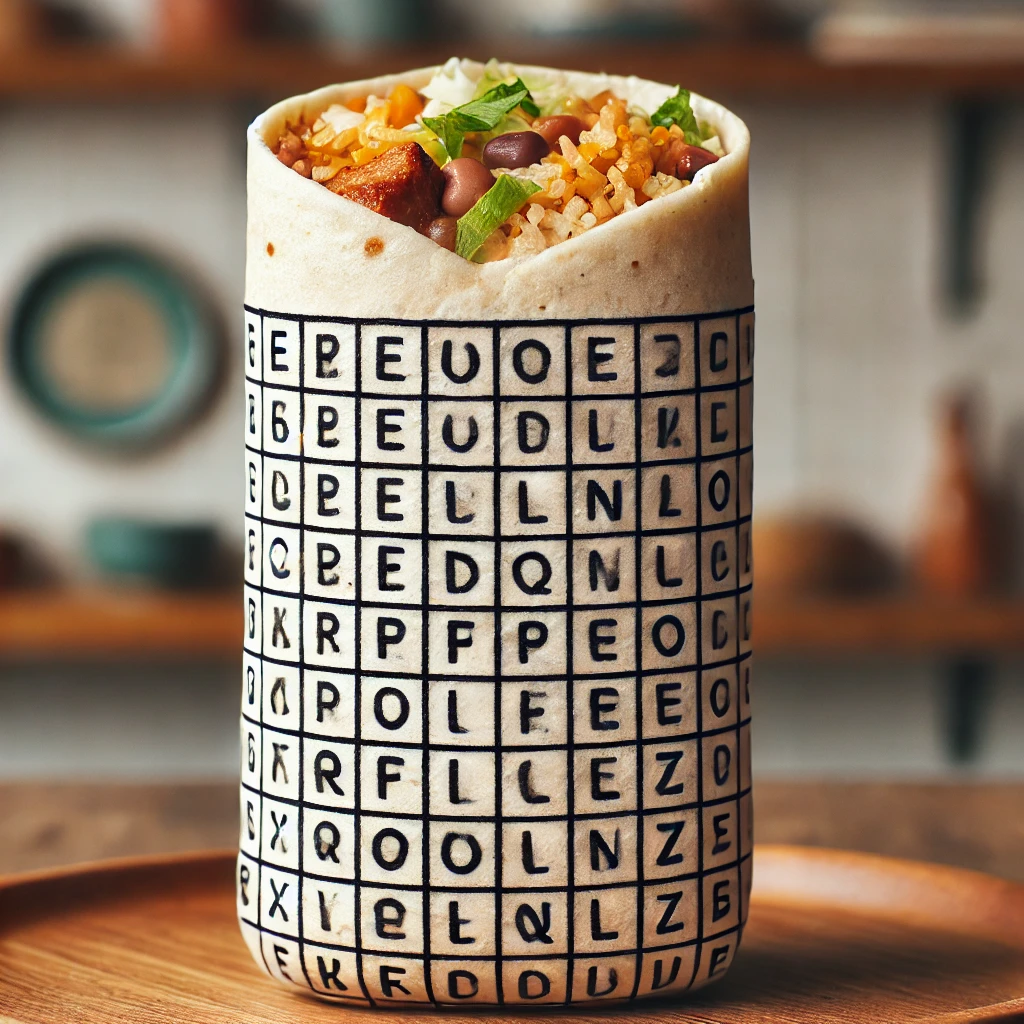
\includegraphics[scale=0.145]{burrito-1.png}
  \caption{Imagen del prototipo presentado durante la convención.}
  \end{figure}
\end{problemDescription}

\begin{inputDescription}
  La primera línea de la entrada contiene un entero $n$ ($2 \leq n \leq 50$) correspondiente
  al tamaño de la cuadrícula.

  Cada una de las siguientes $n$ líneas contiene $n$ caracteres, describiendo
  las filas de la cuadrícula de arriba hacia abajo.

  Luego sigue una línea conteniendo un entero $m$ ($1 \leq m \leq 50$), correspondiente
  a la cantidad de palabras a buscar.

  Cada una de las siguientes $m$ líneas contienen una palabra a buscar.
  %
  El largo de cada una de las palabras a buscar será mayor o igual a 2 y menor o igual
  que $n$.

  Todos los caracteres de la cuadrícula y de las $m$ palabras corresponden a letras mayúsculas
  del alfabeto inglés.
\end{inputDescription}

\begin{outputDescription}
  Para cada una de las $m$ palabras, imprime una línea que diga \texttt{PRESENTE} si la palabra está
  en el burrito de letras o \texttt{AUSENTE} de lo contrario.
\end{outputDescription}

\begin{scoreDescription}
  \subtask{50} Se probarán varios casos en que se garantiza que no aparecen palabras en sentido
  horizontal, es decir, si una palabra está presente, esta aparecerá de forma vertical.
  \subtask{50} Se probarán varios casos de prueba sin restricciones adicionales.
\end{scoreDescription}

\begin{sampleDescription}
\sampleIO{sample-1}
\sampleIO{sample-2}
\end{sampleDescription}

\end{document}
